\documentclass[
	fontsize=12pt,          % default font size 12pt
	paper=a4,               % DIN A4 page format
	numbers=noenddot,       % remove dots behind chapter numbers (e.g. 1.5 not 1.5.)
	listof=totoc,           % add list of figures, tables, etc. to ToC
	listof=entryprefix,     % add entry name to figures, tables, etc.
	listof=nochaptergap,    % no chapter gap for figures, tables, etc.
	bibliography=totoc,     % add bibliography to ToC but without a chapter number
	parskip=half,           % half line spacing between paragraphs
	openany                 % chapters can start on any page
]{scrbook}

\include{../../for_latex/preamble}

\usepackage{tikz}
\usetikzlibrary{positioning, shapes.geometric, arrows.meta, shapes.symbols, fit, calc}
\usepackage{longtable}

\begin{document}

\begin{titlepage}
	\pagestyle{empty}

	% HFU Logo
	\begin{flushright}
		\begin{figure}[ht]
			\flushright
			
\includegraphics[height=2cm]{../../for_latex/hfu}
		\end{figure}
	\end{flushright}

	\begin{center}
		\vspace{3cm}

		{\fontsize{22}{22} \selectfont \textbf{Blatt 4}}\\[5mm]
		{\fontsize{18}{18} \selectfont Software Qualität}\\[3mm]
		{\fontsize{14}{14} \selectfont Softwareanforderungsspezifikation}\\
		{\fontsize{14}{14} \selectfont Schwarzwald-Entdecker}

		\vspace{10cm}

		{\fontsize{14}{14} \selectfont Luis Staudt}
	\end{center}
\end{titlepage}

% ############################################################################
% CONTENT STARTS HERE
% ############################################################################

\chapter*{1. Einleitung}


\section*{1.1 Zweck}

Dieses Dokument beschreibt die funktionalen und nichtfunktionalen Anforderungen an das Portal \emph{Schwarzwald-Entdecker} mit Schwerpunkt auf dem Ausflugs-Konfigurator.
Es dient als Grundlage für Entwurf, Implementierung und Test.


\section*{1.2 Projektumfang}

\emph{Schwarzwald-Entdecker} ist ein Webportal, über das Kunden Aktivitäten und Ausflüge im Schwarzwald filtern, individuell planen und buchen können.
Zentrales Element ist der Konfigurator, der Ausflüge nach Kriterien wie Art, Dauer, Anfangs- und Endzeit sowie Ausflugsort zusammenstellt.


\section*{1.3 Zielgruppen}

\begin{itemize}
	\item \textbf{Gast:} ungebundener Besucher, kann Ausflüge ansehen und filtern.
	\item \textbf{Registrierter Kunde:} kann zusätzlich buchen, Planungen speichern und ändern.
	\item \textbf{Administrator:} pflegt Angebote, Kapazitäten und Stammdaten.
\end{itemize}


\chapter*{2. Gesamtbeschreibung}


\section*{2.1 Produktperspektive}

Das System ist eine eigenständige Webanwendung mit Datenbankanbindung.
Die Oberfläche ist responsiv und auf gängigen Browsern sowie mobilen Geräten nutzbar.


\section*{2.2 Betriebsumgebung}

\begin{itemize}
	\item Clientseite: aktuelle Versionen gängiger Browser (Chrome, Firefox, Safari, Edge), Desktop und mobil.
	\item Serverseite: Webserver mit Anwendungslogik und Datenbankanbindung.
\end{itemize}


\section*{2.3 Annahmen und Abhängigkeiten}

Die Verfügbarkeit der Ausflüge wird über einen externen Anbieterdatenbestand gepflegt.
Zahlungen werden über einen externen Zahlungsdienstleister abgewickelt.


\chapter*{3. Systemfunktionen}


\section*{3.1 Anwendungsfälle (Use Cases)}

Die folgenden drei Anwendungsfälle modellieren die Kerninteraktion des Kunden mit dem Konfigurator.

\subsection*{Use-Case-Diagramm}

\begin{center}
\begin{tikzpicture}[node distance=1.2cm, every node/.style={font=\small}]
	\node (actor) [draw=none] at (0,0) {
		\begin{tikzpicture}
			\draw (0,0) circle (0.2);
			\draw (0,-0.2) -- (0,-0.9);
			\draw (-0.3,-0.4) -- (0.3,-0.4);
			\draw (0,-0.9) -- (-0.25,-1.3);
			\draw (0,-0.9) -- (0.25,-1.3);
		\end{tikzpicture}
	};
	\node[below=0.1cm of actor] {Kunde};

	\node[draw, ellipse, minimum width=3.8cm, minimum height=0.9cm] (uc1) at (5,1.2) {Ausflug konfigurieren};
	\node[draw, ellipse, minimum width=3.8cm, minimum height=0.9cm] (uc2) at (5,0) {Ausflug buchen};
	\node[draw, ellipse, minimum width=3.8cm, minimum height=0.9cm] (uc3) at (5,-1.2) {Mehrtagestour planen};

	\node[draw, fit=(uc1)(uc2)(uc3), inner sep=0.4cm, label=above:\textbf{Konfigurator}] (sys) {};

	\draw (actor) -- (uc1);
	\draw (actor) -- (uc2);
	\draw (actor) -- (uc3);
\end{tikzpicture}
\end{center}


\subsection*{UC-01: Ausflug konfigurieren}

\begin{tabular}{| p{4cm} | p{9.5cm} |}
	\hline
	\textbf{Akteur} & Kunde (Gast oder registriert) \\ \hline
	\textbf{Ziel} & Einen passenden Ausflug nach Vorgaben finden. \\ \hline
	\textbf{Vorbedingung} & Portal ist erreichbar, Angebote sind verfügbar. \\ \hline
	\textbf{Nachbedingung} & Konfigurierter Ausflug wird angezeigt. \\ \hline
	\textbf{Ablauf} & 1. Kunde öffnet Konfigurator.\newline
	                  2. Kunde wählt Art, Dauer, Anfangs- und Endzeit sowie Ort.\newline
	                  3. System filtert verfügbare Ausflüge.\newline
	                  4. System zeigt Trefferliste an. \\ \hline
	\textbf{Ausnahmen} & Kein Treffer: Hinweis mit Vorschlag zur Filteranpassung. \\ \hline
\end{tabular}


\subsection*{UC-02: Ausflug buchen}

\begin{tabular}{| p{4cm} | p{9.5cm} |}
	\hline
	\textbf{Akteur} & Registrierter Kunde \\ \hline
	\textbf{Ziel} & Einen konfigurierten Ausflug verbindlich reservieren. \\ \hline
	\textbf{Vorbedingung} & Kunde ist angemeldet, Ausflug ist konfiguriert. \\ \hline
	\textbf{Nachbedingung} & Buchung ist gespeichert und bestätigt. \\ \hline
	\textbf{Ablauf} & 1. Kunde wählt ,,Buchen''.\newline
	                  2. System prüft Verfügbarkeit.\newline
	                  3. System leitet an Zahlungsdienstleister weiter.\newline
	                  4. System speichert Buchung und sendet Bestätigung. \\ \hline
	\textbf{Ausnahmen} & Nicht verfügbar: Fehlermeldung, Rückkehr zur Konfiguration.\newline
	                     Zahlung fehlgeschlagen: Buchung wird nicht gespeichert. \\ \hline
\end{tabular}


\subsection*{UC-03: Mehrtagestour planen}

\begin{tabular}{| p{4cm} | p{9.5cm} |}
	\hline
	\textbf{Akteur} & Registrierter Kunde \\ \hline
	\textbf{Ziel} & Mehrere Ausflüge zu einer Mehrtagestour zusammenfassen. \\ \hline
	\textbf{Vorbedingung} & Kunde ist angemeldet. \\ \hline
	\textbf{Nachbedingung} & Tour ist zusammengestellt und zur Buchung bereit. \\ \hline
	\textbf{Ablauf} & 1. Kunde startet Tourplanung.\newline
	                  2. Kunde fügt mehrere konfigurierte Ausflüge hinzu.\newline
	                  3. System prüft zeitliche Konsistenz.\newline
	                  4. System zeigt Gesamttour und Preis an. \\ \hline
	\textbf{Ausnahmen} & Zeitliche Überschneidung: Warnung und Vorschlag zur Anpassung. \\ \hline
\end{tabular}


\section*{3.2 User Stories (Story-Card-Methode)}

\subsection*{US-01: Ausflug filtern}

\begin{tabular}{| p{4cm} | p{9.5cm} |}
	\hline
	\textbf{Story} & Als Kunde möchte ich Ausflüge nach Art, Dauer und Ort filtern, damit ich schnell passende Angebote finde. \\ \hline
	\textbf{Akzeptanzkriterien} &
	$\bullet$ Filter für Art, Dauer, Anfangs-/Endzeit und Ort sind verfügbar.\newline
	$\bullet$ Nur verfügbare Ausflüge werden angezeigt.\newline
	$\bullet$ Bei keinem Treffer erscheint ein Hinweis. \\ \hline
	\textbf{Priorität} & Hoch \\ \hline
\end{tabular}


\subsection*{US-02: Buchung abschließen}

\begin{tabular}{| p{4cm} | p{9.5cm} |}
	\hline
	\textbf{Story} & Als registrierter Kunde möchte ich einen konfigurierten Ausflug buchen, damit meine Reservierung verbindlich ist. \\ \hline
	\textbf{Akzeptanzkriterien} &
	$\bullet$ Verfügbarkeit wird vor Bezahlung geprüft.\newline
	$\bullet$ Nach erfolgreicher Zahlung wird die Buchung gespeichert.\newline
	$\bullet$ Kunde erhält eine Bestätigung per E-Mail. \\ \hline
	\textbf{Priorität} & Hoch \\ \hline
\end{tabular}


\subsection*{US-03: Mehrtagestour zusammenstellen}

\begin{tabular}{| p{4cm} | p{9.5cm} |}
	\hline
	\textbf{Story} & Als Kunde möchte ich mehrere Ausflüge zu einer Mehrtagestour kombinieren, damit meine Urlaubsplanung erhalten bleibt. \\ \hline
	\textbf{Akzeptanzkriterien} &
	$\bullet$ Mehrere Ausflüge können einer Tour hinzugefügt werden.\newline
	$\bullet$ Zeitliche Überschneidungen werden erkannt und gemeldet.\newline
	$\bullet$ Die Planung bleibt nach Abmeldung erhalten. \\ \hline
	\textbf{Priorität} & Mittel \\ \hline
\end{tabular}


\section*{3.3 Aktivitätsdiagramm: Konfigurieren und Buchen}

\begin{center}
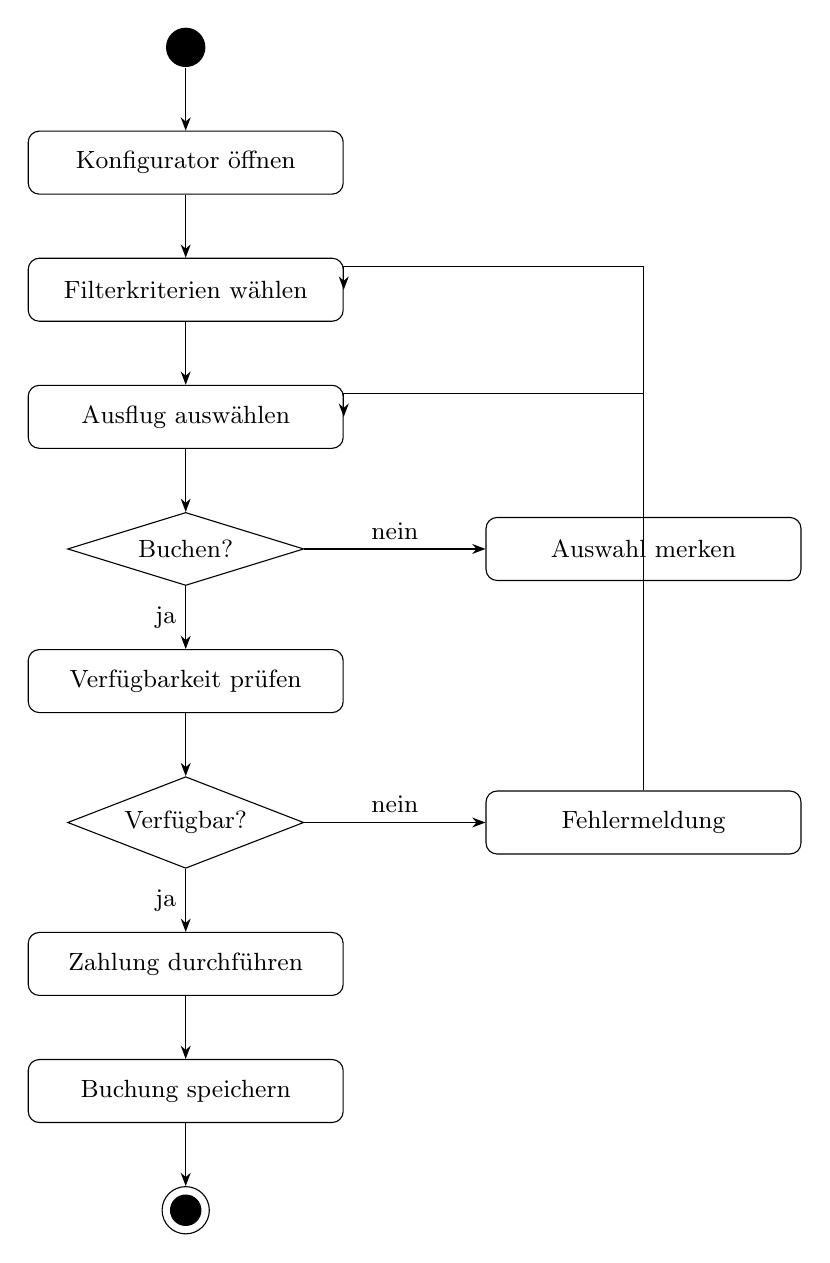
\begin{tikzpicture}[
	node distance=0.8cm and 1cm,
	start/.style={circle, fill=black, minimum size=5mm},
	stop/.style={circle, draw, minimum size=6mm, path picture={\fill (path picture bounding box.center) circle (2mm);}},
	action/.style={rectangle, rounded corners, draw, minimum width=4cm, minimum height=0.8cm, align=center},
	decision/.style={diamond, draw, aspect=2, minimum width=3cm, align=center, inner sep=1pt},
	arrow/.style={-Stealth},
	every node/.style={font=\small}
]
	\node[start] (s) {};
	\node[action, below=of s] (a1) {Konfigurator öffnen};
	\node[action, below=of a1] (a2) {Filterkriterien wählen};
	\node[action, below=of a2] (a3) {Ausflug auswählen};
	\node[decision, below=of a3] (d1) {Buchen?};
	\node[action, below=of d1] (a4) {Verfügbarkeit prüfen};
	\node[decision, below=of a4] (d2) {Verfügbar?};
	\node[action, below=of d2] (a5) {Zahlung durchführen};
	\node[action, below=of a5] (a6) {Buchung speichern};
	\node[stop, below=of a6] (e) {};

	\node[action, right=2.3cm of d1] (nop) {Auswahl merken};
	\node[action, right=2.3cm of d2] (warn) {Fehlermeldung};

	\draw[arrow] (s) -- (a1);
	\draw[arrow] (a1) -- (a2);
	\draw[arrow] (a2) -- (a3);
	\draw[arrow] (a3) -- (d1);
	\draw[arrow] (d1) -- node[left]{ja} (a4);
	\draw[arrow] (d1) -- node[above]{nein} (nop);
	\draw[arrow] (a4) -- (d2);
	\draw[arrow] (d2) -- node[left]{ja} (a5);
	\draw[arrow] (d2) -- node[above]{nein} (warn);
	\draw[arrow] (a5) -- (a6);
	\draw[arrow] (a6) -- (e);
	\draw[arrow] (warn.north) |- ([yshift=3mm]a3.east) -- (a3.east);
	\draw[arrow] (nop.north) |- ([yshift=3mm]a2.east) -- (a2.east);
\end{tikzpicture}
\end{center}


\chapter*{4. Datenanforderungen}


\section*{4.1 Wesentliche Datenobjekte}

\begin{tabular}{| p{3.5cm} | p{10cm} |}
	\hline
	\textbf{Entität} & \textbf{Wesentliche Attribute} \\ \hline
	Kunde & ID, Name, E-Mail, Passwort-Hash, Adresse, Rolle \\ \hline
	Ausflug & ID, Art, Ort, Anfangs-/Endzeit, Dauer, Preis, Kapazität \\ \hline
	Aktivität & ID, Name, Beschreibung, Anbieter \\ \hline
	Buchung & ID, KundenID, AusflugID, Datum, Status, Zahlungsreferenz \\ \hline
	Mehrtagestour & ID, KundenID, Liste von AusflugIDs, Gesamtpreis \\ \hline
\end{tabular}


\section*{4.2 Datenhaltung}

\begin{itemize}
	\item Persistente Speicherung in einer relationalen Datenbank.
	\item Temporäre Planungsdaten werden mit dem Kundenkonto verknüpft und bleiben auch nach Abmeldung erhalten.
	\item Personenbezogene Daten werden gemäß DSGVO verschlüsselt gespeichert.
\end{itemize}


\chapter*{5. Anforderungen an externe Schnittstellen}


\section*{5.1 Benutzungsschnittstelle}

\begin{itemize}
	\item Responsive Weboberfläche für Desktop und mobile Geräte.
	\item Barrierearme Bedienung, konsistente Navigation, klare Fehlermeldungen.
	\item Unterstützung aktueller Versionen von Chrome, Firefox, Safari und Edge.
\end{itemize}


\section*{5.2 Softwareschnittstellen}

\begin{itemize}
	\item Datenbank: Anbindung über ein ORM oder SQL-API.
	\item Zahlungsdienstleister: REST-API für Bezahlvorgänge.
	\item E-Mail-Dienst: SMTP-API für Buchungsbestätigungen.
\end{itemize}


\section*{5.3 Kommunikationsschnittstellen}

\begin{itemize}
	\item HTTPS für alle Clientverbindungen (TLS 1.2 oder höher).
	\item REST über HTTPS für externe Services.
\end{itemize}


\chapter*{6. Nichtfunktionale Anforderungen}


\section*{6.1 Performance}

\begin{itemize}
	\item Antwortzeit für Filterabfragen $\leq$ 2 Sekunden bei durchschnittlicher Last.
	\item System unterstützt mindestens 500 gleichzeitige Nutzer ohne spürbare Verzögerung.
\end{itemize}


\section*{6.2 Verfügbarkeit und Zuverlässigkeit}

\begin{itemize}
	\item Verfügbarkeit mindestens 99\,\% im Jahresmittel.
	\item Transaktionssichere Buchung: keine Teilbuchungen bei Fehlern.
\end{itemize}


\section*{6.3 Sicherheit und Datenschutz}

\begin{itemize}
	\item Passwörter werden ausschließlich als Hash mit Salt gespeichert.
	\item Zahlungsdaten werden nicht im System gespeichert.
	\item Verarbeitung personenbezogener Daten gemäß DSGVO.
\end{itemize}


\section*{6.4 Benutzbarkeit}

\begin{itemize}
	\item Eine Buchung ist in maximal fünf Schritten abschließbar.
	\item UI-Texte sind auf Deutsch, Erweiterbarkeit auf weitere Sprachen vorgesehen.
\end{itemize}


\section*{6.5 Wartbarkeit und Portierbarkeit}

\begin{itemize}
	\item Modularer Aufbau mit klar getrennten Schichten (Präsentation, Logik, Datenhaltung).
	\item Betrieb auf gängigen Linux-Servern, Containerisierung möglich.
\end{itemize}


\chapter*{7. Weitere funktionale Anforderungen}

Die folgenden Anforderungen sind gemäß den Qualitätsmaßen nach C.~Rupp formuliert (eindeutig, vollständig, verifizierbar, atomar).

\begin{longtable}{| p{1.6cm} | p{12cm} |}
	\hline
	\textbf{ID} & \textbf{Anforderung} \\ \hline
	\endfirsthead
	\hline
	\textbf{ID} & \textbf{Anforderung} \\ \hline
	\endhead
	\hline
	\endfoot

	FA-01 & Das System muss dem Kunden die Registrierung mit E-Mail-Adresse und Passwort ermöglichen. \\ \hline
	FA-02 & Das System muss dem registrierten Kunden die Anmeldung über E-Mail und Passwort ermöglichen. \\ \hline
	FA-03 & Das System soll dem registrierten Kunden die Bearbeitung seines Profils (Name, Adresse, E-Mail) ermöglichen. \\ \hline
	FA-04 & Das System muss dem Kunden die Übersicht aller vergangenen und zukünftigen Buchungen anzeigen. \\ \hline
	FA-05 & Das System muss dem Kunden das Stornieren einer Buchung bis 24 Stunden vor Beginn ermöglichen. \\ \hline
	FA-06 & Das System soll dem Kunden das Ändern einer Buchung (Datum, Teilnehmerzahl) ermöglichen, sofern verfügbar. \\ \hline
	FA-07 & Das System muss die Planung eines konfigurierten Ausflugs dauerhaft mit dem Kundenkonto verknüpfen. \\ \hline
	FA-08 & Das System muss nach erfolgreicher Buchung eine Bestätigung per E-Mail versenden. \\ \hline
	FA-09 & Das System muss dem Administrator die Pflege der Ausflugs- und Kapazitätsdaten ermöglichen. \\ \hline
	FA-10 & Das System muss ungültige Eingaben (z.\,B.\ leere Pflichtfelder) erkennen und eine verständliche Fehlermeldung anzeigen. \\ \hline
\end{longtable}


% ############################################################################
% CONTENT ENDS HERE
% ############################################################################

\end{document}
